\documentclass{article} % For LaTeX2e
\usepackage{nips14submit_e,times}
\usepackage{hyperref}
\usepackage{url}
\usepackage{graphicx}
\usepackage{algorithm}
\usepackage{amsmath}


\usepackage[noend]{algpseudocode}
\usepackage{subcaption}
%\documentstyle[nips14submit_09,times,art10]{article} % For LaTeX 2.09


\title{Latent Dirichlet Analysis for Document Topic Modelling}


\author{
Xiang Li\\
%Department of Computer Science
%University of Michigan\\
%Ann Arbor, MI 48109 \\
\texttt{xngli@umich.edu} \\
\And
Zheng Luo \\
%University of Michigan\\
%Ann Arbor, MI 48109 \\
\texttt{zluo@umich.edu} \\
\AND
Yan Chen\\
%University of Michigan\\
%Ann Arbor, MI 48109 \\
\texttt{yanchenm@umich.edu} \\
\And
Sajan Patel\\
%University of Michigan\\
%Ann Arbor, MI 48109\\
\texttt{sajanptl@umich.edu} \\
}

% The \author macro works with any number of authors. There are two commands
% used to separate the names and addresses of multiple authors: \And and \AND.
%
% Using \And between authors leaves it to \LaTeX{} to determine where to break
% the lines. Using \AND forces a linebreak at that point. So, if \LaTeX{}
% puts 3 of 4 authors names on the first line, and the last on the second
% line, try using \AND instead of \And before the third author name.

\newcommand{\fix}{\marginpar{FIX}}
\newcommand{\new}{\marginpar{NEW}}

\nipsfinalcopy % Uncomment for camera-ready version


\makeatletter
\def\BState{\State\hskip-\ALG@thistlm}
\makeatother

\begin{document}



\maketitle

\begin{abstract}
In this project, we studied the topic latent Dirichlet allocation (LDA), a nonparametric Bayesian model for collections of discrete data such as text corpora, which was first proposed by Blei, Ng, and Jordan in 2003 [1]. We followed the original paper to implement LDA using variance inference techniques and an EM algorithm for estimating the Bayes parameters and extracting subtopic from a text corpus. In addition, we also implemented LDA using collapsed Gibbs Sampling following Griffiths and Steyvers (2004). We recreated the document modeling experiment in [1] to extract subtopics on AP dataset. It was found variational inference and Gibbs sampling generated similar perplexities and subtopics. We also compared LDA with simple unigram model (and find that ... ).

%The abstract paragraph should be indented 1/2~inch (3~picas) on both left and
%right-hand margins. Use 10~point type, with a vertical spacing of 11~points.
%The word \textbf{Abstract} must be centered, bold, and in point size 12. Two
%line spaces precede the abstract. The abstract must be limited to one
%paragraph.
\end{abstract}

\section{Introduction}
Here, describe the problem statement: Given a text document, model the topics of the document. (expand on that more).

\subsection{Related Works}
Based on Blei, briefly talk about unigram, mixture of unigram, and plsi.

\section{Notation}
We used similar notation as those denoted in the paper: \\
$K$ = number of topics\\
$D$ = number of documents\\
$V$ = vocabulary size\\
$N$ =  number of words in total.\\
$z_j$ = the j-th topic\\
$d_i$ = the i-th document\\
$w_i$ = the i-th word in the document\\

\section{LDA}
The latent Dirichlet allocation (LDA) model explains the generation of text documents, which can be viewed as samples from a mixture of multinomial distributions over a vocabulary of words. Each multinomial mixture component is called a “topic”. The general process of the model to write a document is the following:

\begin{itemize}
\item The number of words $N$ in document $\sim$ Poisson ($\zeta$)
\item The topic mixture $\theta$ for the document $\sim$ Dir ($\alpha$) (with a fixed set of $K$ topics)
\item Then for each word $w_i$ in the document:
\begin{enumerate}
\item Choose a topic $t_i$ based on multinomial distribution with parameter $\theta$ from step (2)
\item Use this topic $z_i$ to generate word itself by using the existing probability for each word in this topic (i.e. $p(w_i | z_i, \beta)$
\end{enumerate}
\end{itemize}

\begin{figure}
    \centering
    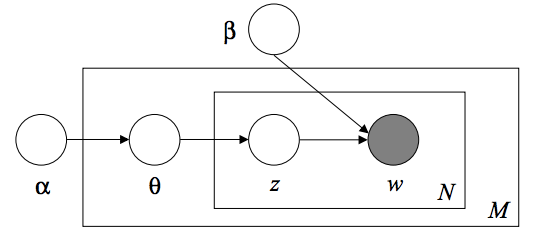
\includegraphics[width=0.6\textwidth]{graphmodel}
    \caption{Graphic model of LDA. The boxes are ``plates'' representing replicates. The outer plate represents documents, while the inner plate represents the repeated choice of topics and words within a document.}
    \label{fig:graphmodel}
\end{figure}


This is the generative model for a collection of documents. LDA then tries to backtrack from the (training) documents to find a set of topics that are likely to have generated the collection. Now the question is how does LDA backtrack to find the parameters in this model. Suppose we have a set of documents D, and we set the number of topics to be K. What we want is to use LDA to learn two things 1) the topic representation of each document and 2) the words associated to each topic.

There are two methods to learn these two things: collapsed Gibbs sampling [1] and variational inference [2, 3]. We first discuss Gibbs sampling method here:


\subsection{Gibbs Sampling Method}
\begin{itemize}
\item For each document, randomly assign each word in the document to one of the $K$ topics.
\begin{enumerate}
\item this step gives topic representation of all the documents
\item this step gives word distributions of all the topics
\item since randomly assign topics to each word is very native, so we need to improve it
\end{enumerate}
\item For each word $w_k$ in document $d_i$
\begin{enumerate}
\item For each topic $t_j$ that this word belongs to, compute:
\begin{enumerate}
\item $p(z_j | d_i)  = \frac{number of words assigned to z_j in d_i}{total number of words in d_i}$
\item $p( w_k |  z_j) = \frac{number of words assigned to z_j in d_i}{number of words assigned to z_j for all docs}$
\end{enumerate}
\end{enumerate}
\item we compute the product of i) and ii) above which gives the new topics to assign to this word.
\item repeating step 2 over and over until it reaches a steady state where the assignments make good sense.
\item Use this model to estimate the topic mixtures of each document and words associated to each topic, which are the two things we want to learn.
\end{itemize}



\subsection{Inference Method}
With the same Dirichlet distribution model assumption shown in the previous section, variational parameters ($\gamma$ and $\phi$) are introduced. The way to do this is to place a distribution q over hidden variables ($\theta$ and Z) with free parameters which are the so called variational parameters. Then, an optimization process can be performed to make the placed distribution close to the posterior in KL divergence. However, since the KL divergence is intractable, Jensen's inequality is applied to yield an evidence lower bound. Minimizing the KL divergence is equivalent to maximizing the evidence lower bound [5]. The posterior distribution can be obtained with those variational parameters using EM algorithm.

\begin{algorithm}
\caption{Estimation}\label{E-step}
\begin{algorithmic}
\Procedure{}{}
\BState Initializatize: $\phi_{ni}^{0} = 1/K$ for all $i$ and $n$
\BState Initializatize: $\gamma_{i}^{0} = \alpha_i + N/K$ for all $i$
\BState repeat
\For {$n=1$ to $N$}
\For {$i=1$ to $K$}
\State $\phi_{ni}^{t+1}:=\beta_{iw_n}\exp\{\varphi(\gamma_{i}^{t})-\varphi(\sum_{j=1}^{K} \gamma_{j}^{t})\}$
\EndFor {\textbf{end}}
\EndFor {\textbf{end}}
\State $\gamma^{t+1}:=\alpha +\sum_{n=1}^{N}\phi_{n}^{t+1}$
\State $t \gets t+1$
\BState until convergence
\EndProcedure
\end{algorithmic}
\end{algorithm}

\begin{algorithm}
\caption{Maximization}\label{M-step}
\begin{algorithmic}
\Procedure{}{}
\BState Update $\beta$
\For {$i=1$ to $K$}
\For {$j=1$ to $V$}
\State $\beta_{ij} \propto \sum_{d=1}^{D}\sum_{n=1}^{N_d}\phi_{dni}w_{dn}^{j}$
\EndFor {\textbf{end}}
\EndFor {\textbf{end}}
\BState repeat
\State Caculate gradient $g(\alpha^{t})$ and Hessian $H(\alpha^{t})$
\State $\alpha^{t+1} = \alpha^{t} - H^{-1}(\alpha^{t})g(\alpha^{t})$
\State $t \gets t+1$
\BState until convergence

\EndProcedure
\end{algorithmic}
\end{algorithm}


%
%\BState \emph{top}:
%\If {$i > \textit{stringlen}$} \Return false
%\EndIf
%\State $j \gets \textit{patlen}$
%\BState \emph{loop}:
%\If {$\textit{string}(i) = \textit{path}(j)$}
%\State $j \gets j-1$.
%\State $i \gets i-1$.
%\State \textbf{goto} \emph{loop}.
%\State \textbf{close};
%\EndIf
%\State $i \gets i+\max(\textit{delta}_1(\textit{string}(i)),\textit{delta}_2(j))$.
%\State \textbf{goto} \emph{top}.
%\EndProcedure
%\end{algorithmic}
%\end{algorithm}

In the maximization step, the gradient $g(\alpha^{t})$ and Hessian $H(\alpha^{t})$ are calculated using the evidence lower bound $L(\gamma,\phi;\alpha,\beta)$. When applying LDA to training documents, the estimation and maximization steps are iteratively applied until the convergence of the evidence lower bound (or equivalently, until the convergence of perplexity $e^{-L/N}$).

\section{Our Implementation}
\begin{figure}
    \centering
    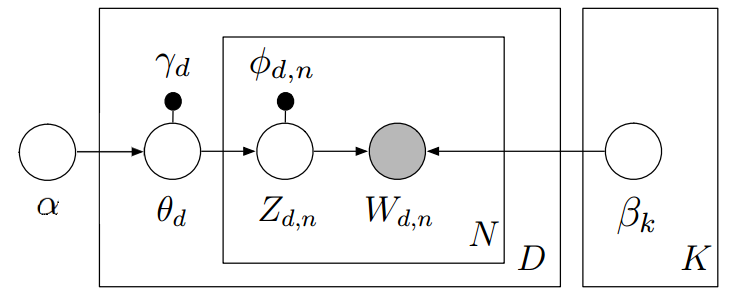
\includegraphics[width=0.6\textwidth]{vi}
    \caption{Graphical model representation of the variational distribution used to approximate the posterior in LDA.}
    \label{fig:graphmodel}
\end{figure}


\section{Evaluations and Empirical Results}
\subsection{Dataset and Preprocessing}
To evaluate our algorithm, we replicated one of the experiments implemented by Blei et al. on document modeling. We used AP dataset which contains 2246 (verify this number) news articles from the associated press [6]. The dataset was partitioned into 80 percent training set and 20 percent test data. In preprocessing of the data, we removed a list of stop words from the text. We further removed words that appear less than 20 times (rare words), as well as words that appear in more than 90 percent of the documents (common words). We ended up with a vocabulary size of 3564.

\subsection{Convergence of Algorithms}
In AP dataset, each document is unlabeled. Therefore, here we are doing unsupervised learning with a purpose to estimate the likelihood of the test dataset. In natural language processing, the likelihood of a document is usually called perplexity, which is the inverse of the average per-word log likelihood. The perplexity of on the text corpus is defined by

Describe perplexity here:

\begin{align*}
perplexity(D_{test}) &= \exp\Big\{{-\frac{\sum_{d=1}^{M} \log{p(w_d)}}{\sum_{d=1}^{M}N_d}}\Big\}\\
& = \exp \Big\{ -\frac{1}{N}\sum_{d=1}^{D}\sum_{i=1}^{N_d}N_{di}\log \sum_{k=1}^{K}\theta_{w_{di}, k}\phi_{d,k} \Big\}
\end{align*}

$$\text{where, }\theta_{v,k} = \frac{C_{vk}+\beta}{\sum_{v'}C_{v' k}+\beta}, \phi_{d,k} = \frac{C_{dk+\alpha}}{\sum_{k'}C_{dk'}+K\alpha}$$


While implementing our algorithms, we first monitors the convergence of the algorithm. This was done by monitoring the perplexity (defined below) of training data, as shown Figure 3. We can see that in both cases the algorithm converges after enough number of iterations, although the numbers of iterations required to reach convergence are very different. Variational inference LDA usually converges after about 10 iteration, while Gibbs sampling LDA needs several hundred. This is a primary reason that the variational inference algorithm is much faster and more commonly used in practice.

\subsection{Extracted Subtopics}
We trained a 10-topic LDA model on the training dataset using both Gibbs sampling and variational inference, and 5 of the generated subtopics in shown in Figure 4. For each topic, the 10 words that are most likely to occur is listed. As we expected, LDA automatically generated meaning full subtopics from the AP corpus, with similar words more likely to appear in the same topic. We also note that the choice and order of words in the topic generated by Gibbs sampling and variational inference are different, although the topics they represented are similar. We think this discrepancy is because the two algorithms we used might converge into different local opitma, and each algorithm used (different) random initialization.


\begin{figure}
\begin{subfigure}{.5\linewidth}
\centering
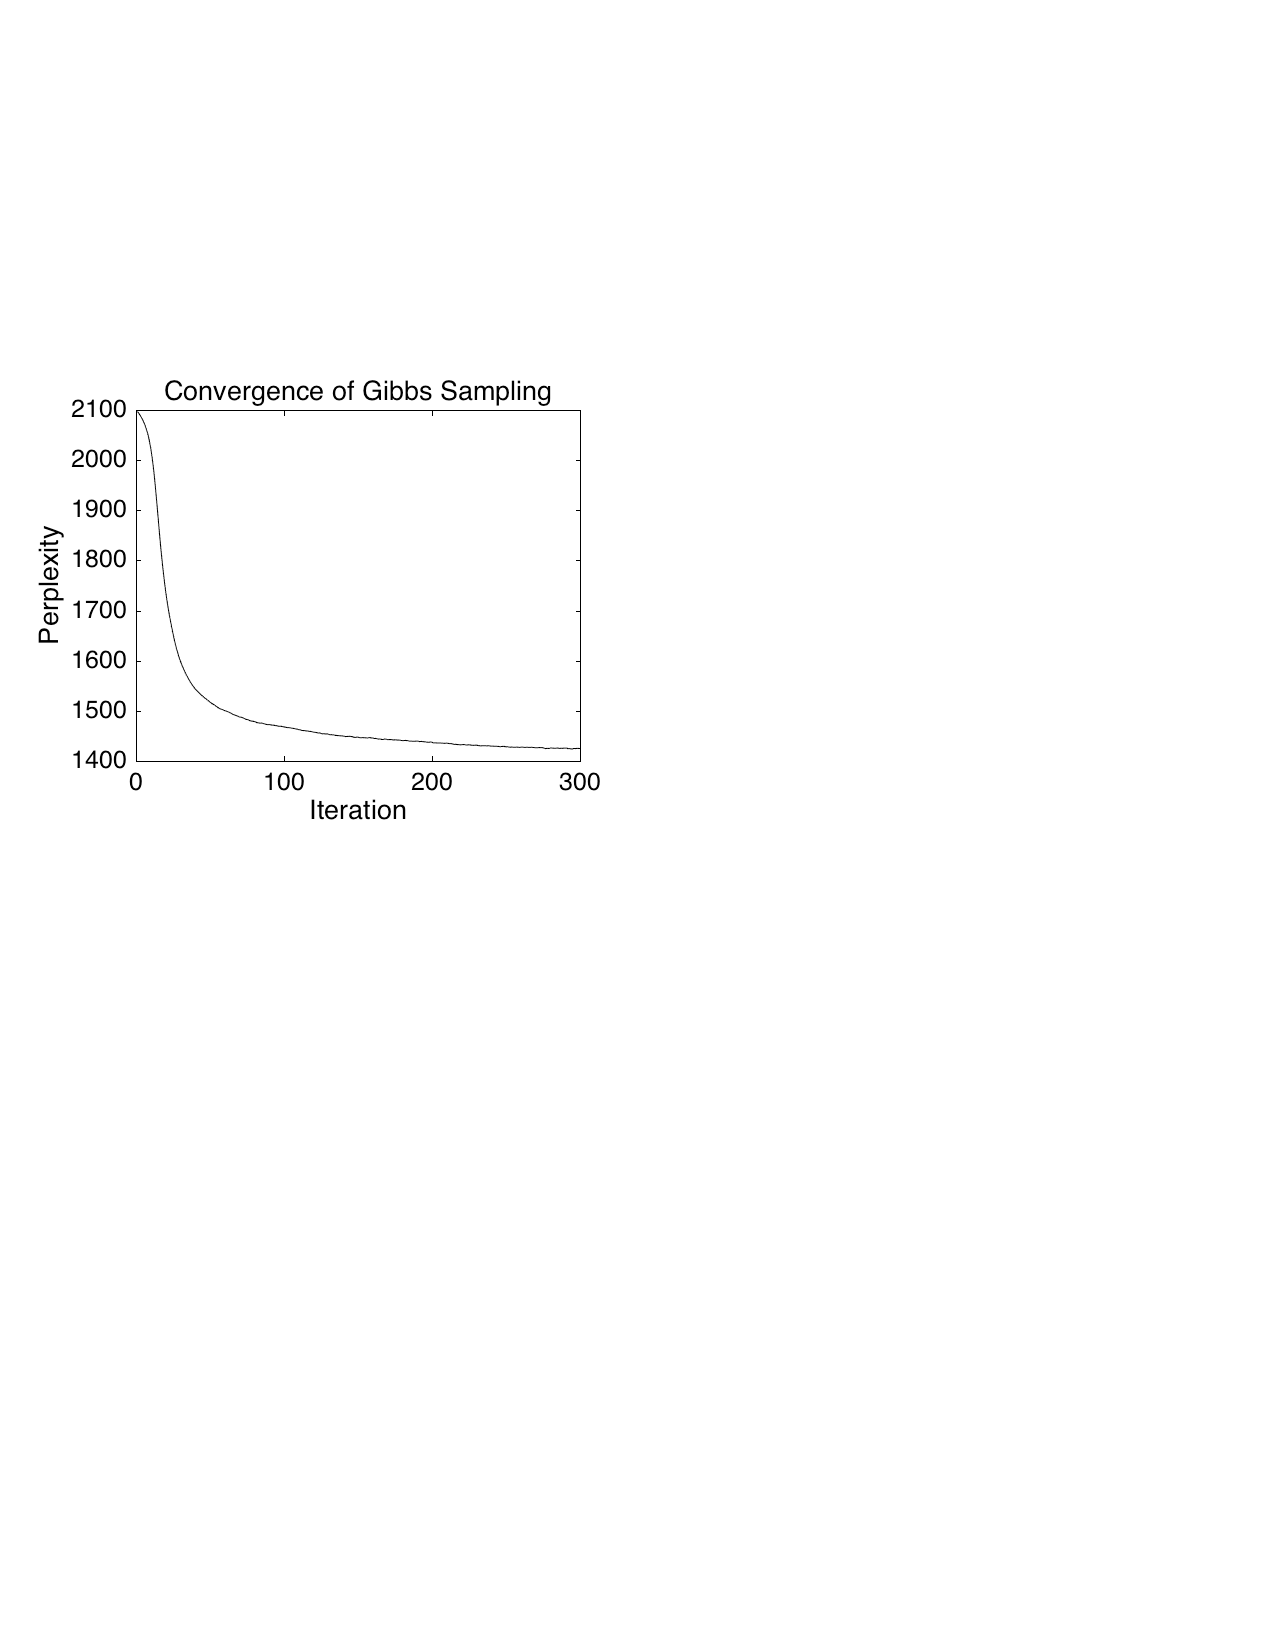
\includegraphics[width=1\textwidth]{AP_topics_10_GS_Perplexity}
\end{subfigure}%
\begin{subfigure}{.5\linewidth}
\centering
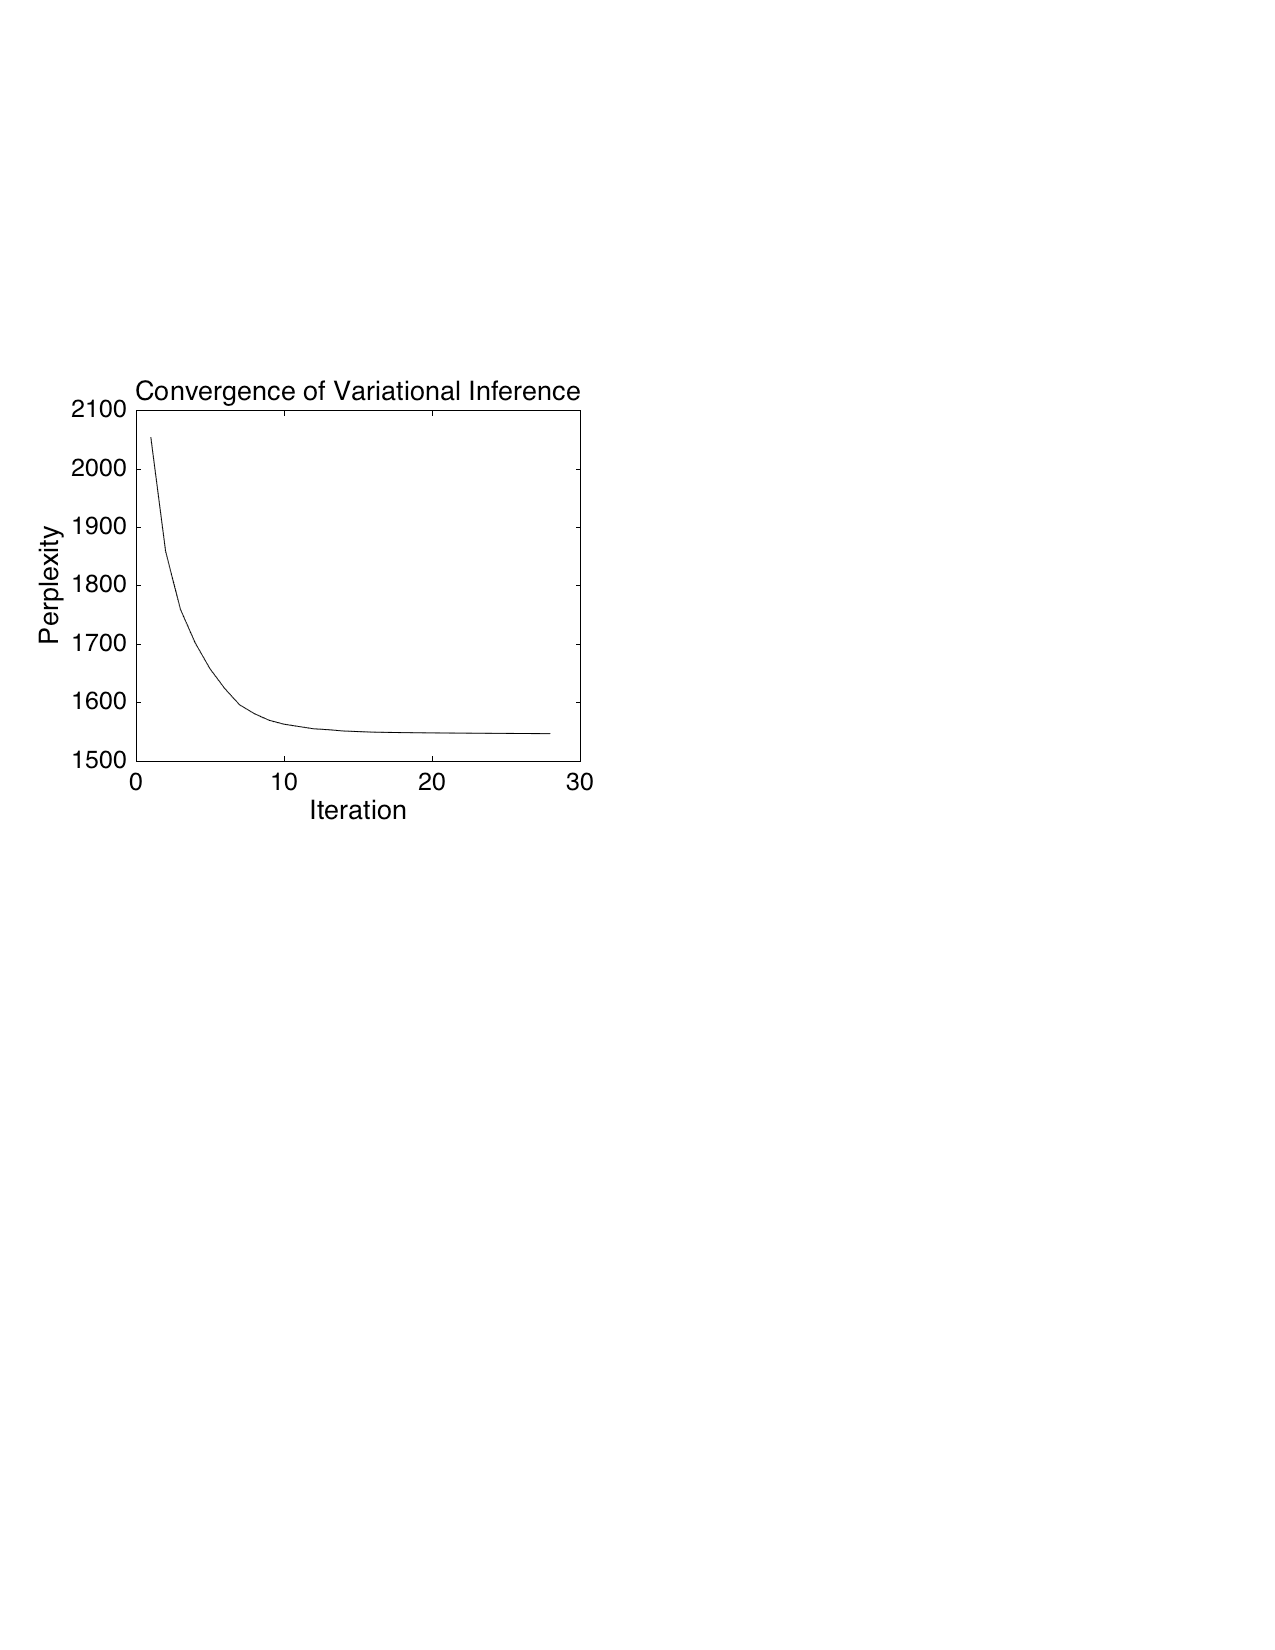
\includegraphics[width=1\textwidth]{AP_topics_10_VI_Perplexity}
\end{subfigure}
\caption{Convergence of LDA using Gibbs Sampling (\textit{left}) and Variational Inference (\textit{right})}\label{fig:convergence}
\end{figure}


\begin{figure}
\begin{subfigure}{1\linewidth}
\centering
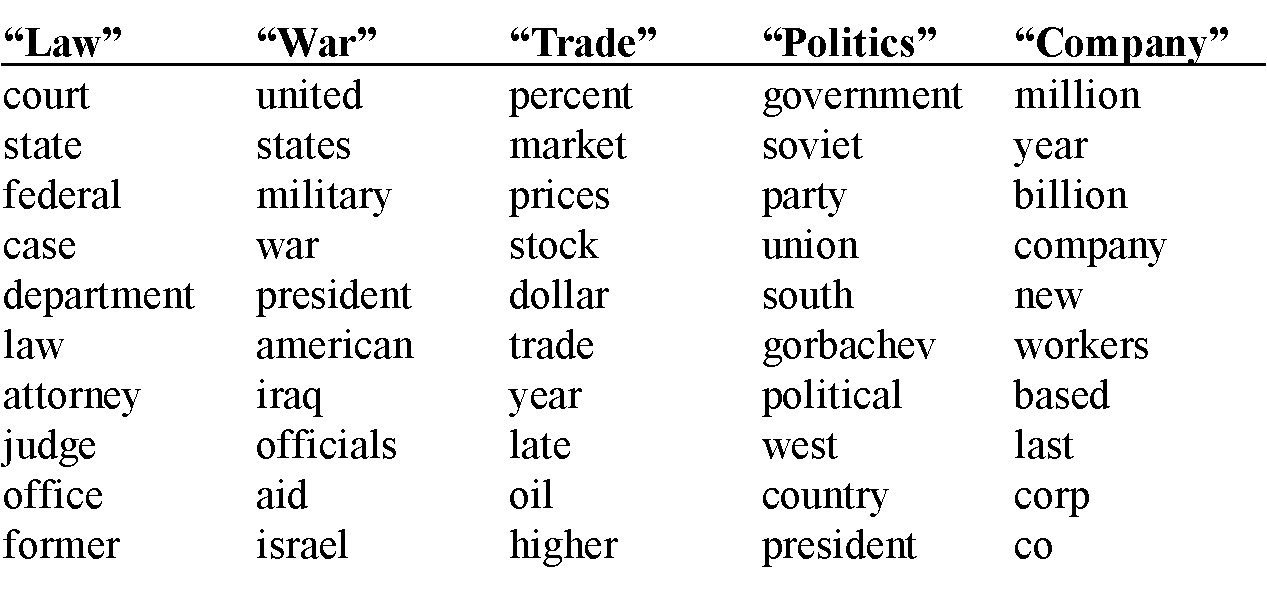
\includegraphics[width=0.8\textwidth]{topics_gs}
\caption{List of topics generated by Gibbs sampling.}
\vspace{1em} %5mm vertical space
\end{subfigure}

\begin{subfigure}{1\linewidth}
\centering
 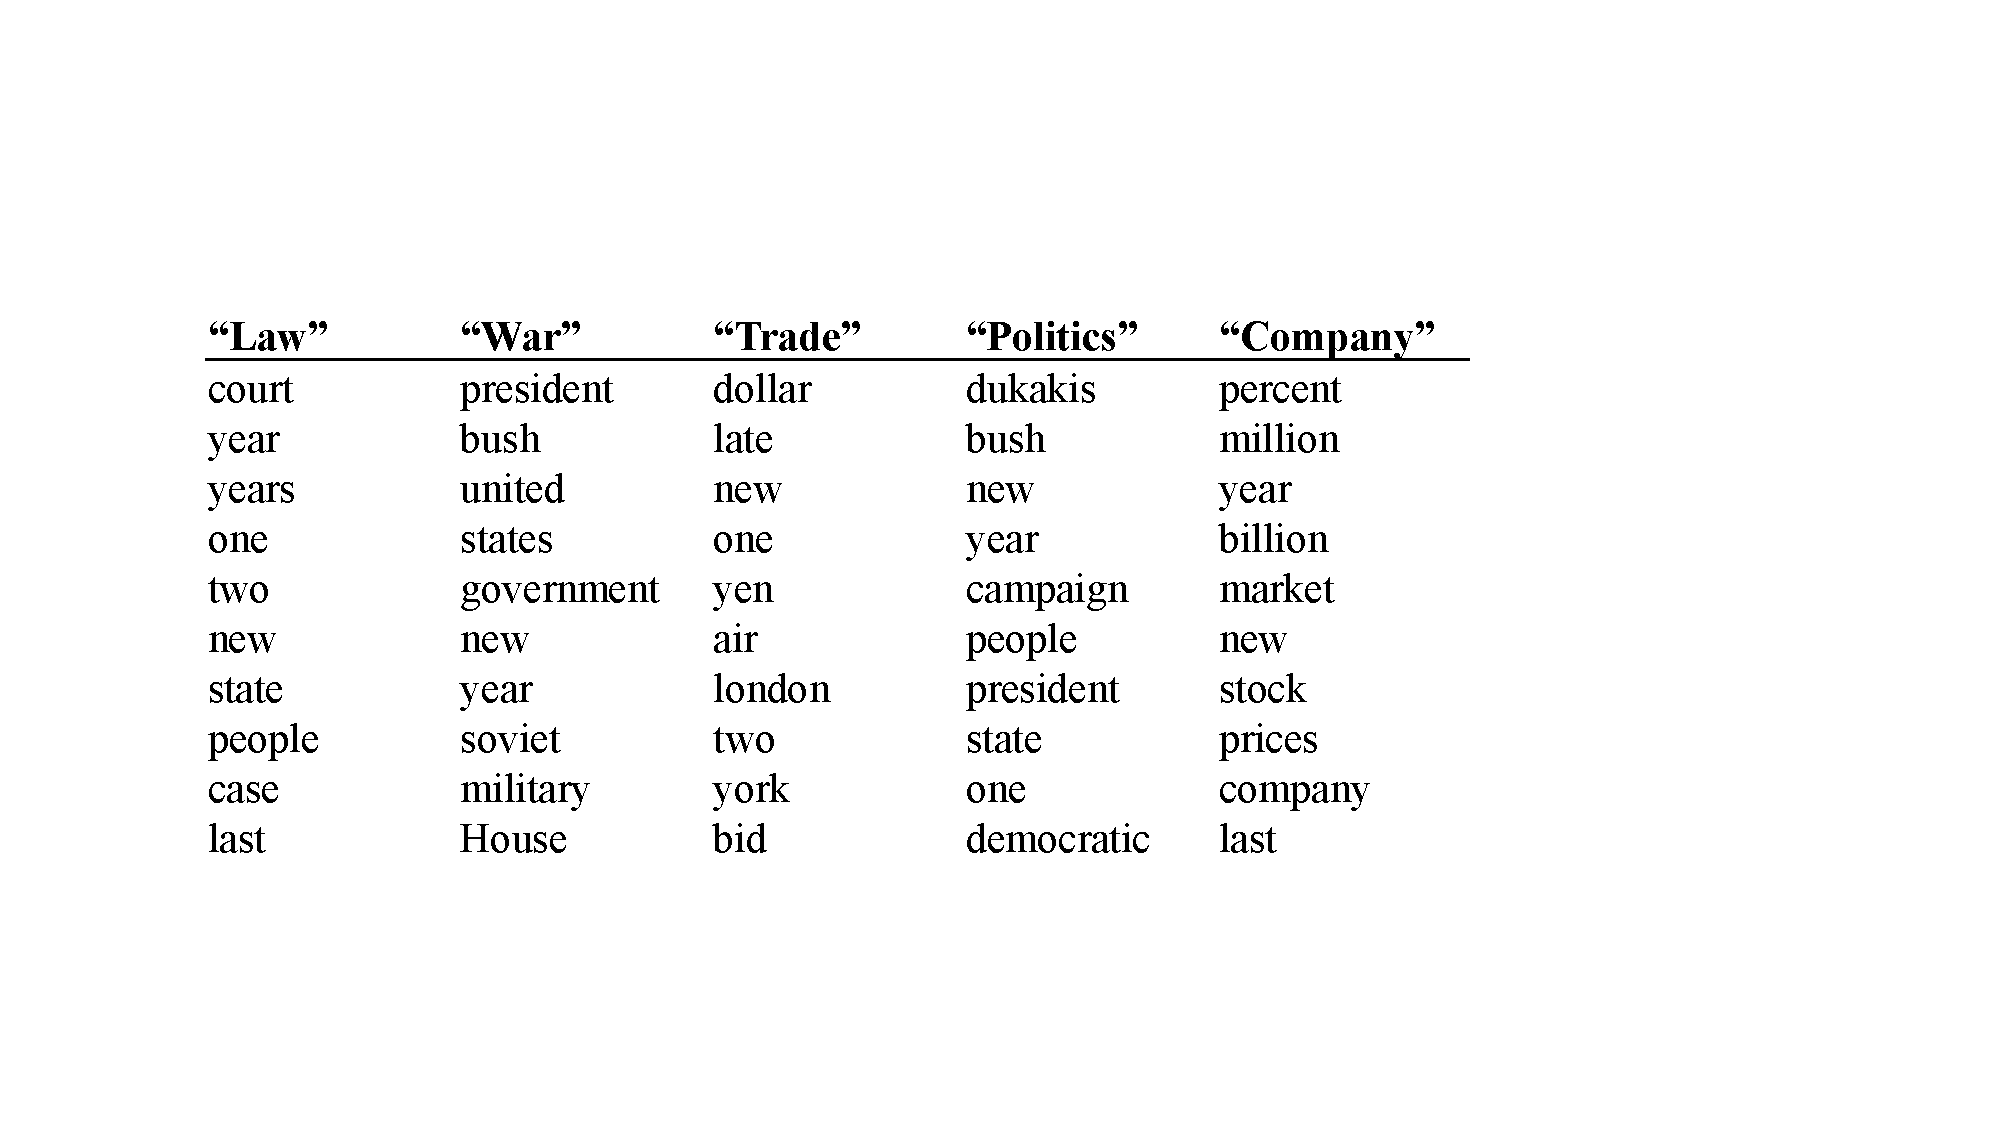
\includegraphics[width=0.8\textwidth]{topics_vi}
 \caption{List of topics generated by variational inference.}
\end{subfigure}
\caption{List of topics generated by LDA using two difference algorithms.}
\label{fig:topics_gs}
\end{figure}

\section{Conclusion}
Discuss the subsequent conclusions we gained from this reimplementation of LDA.
Summarize advantages and disadvantages as well.

%\subsubsection*{Acknowledgments}
%
%Use unnumbered third level headings for the acknowledgments. All
%acknowledgments go at the end of the paper. Do not include
%acknowledgments in the anonymized submission, only in the
%final paper.

\subsubsection*{Author Contributions}
All authors contributed to the overall study of LDA and its implementation. Xiang preprocessed AP dataset in Python to generate input matrices for LDA, and implemented Gibbs Sampling LDA in MATLAB. Zheng implemented variational inference LDA in MATLAB. Sajan implemented the Unigram model in MATLAB. Yan wrote MATLAB functions for calculating perplexity and extracting subtopics from LDA outputs. All authors participated in final data analysis and interpretation, as well as writing of the manuscript.

\subsubsection*{References}

%References follow the acknowledgments. Use unnumbered third level heading for
%the references. Any choice of citation style is acceptable as long as you are
%consistent. It is permissible to reduce the font size to `small' (9-point)
%when listing the references. {\bf Remember that this year you can use
%a ninth page as long as it contains \emph{only} cited references.}

\small{

[1] Griffiths, TL., Steyvers, M. "Finding scientific topics." Proceedings of the National Academy of Sciences.  101(suppl 1) (2004): 5228-35.

[2]. Jordan, Michael I., et al. "An introduction to variational methods for graphical models." Machine Learning 37.2 (1999): 183-233.

[3]. Teh, Yee Whye, et al. "Hierarchical Dirichlet Processes." Journal of the American Statistical Association 101.476 (2006).

[4]. Blei, David M., Andrew Y. Ng, and Michael I. Jordan. "Latent Dirichlet Allocation." the Journal of Machine Learning Research 3 (2003): 993-1022.

[5]. D. Blei and J. Lafferty. "Topic Models." In A. Srivastava and M. Sahami, editors, Text Mining: Classification, Clustering, and Applications. Chapman $\&$ Hall/CRC Data Mining and Knowledge Discovery Series, 2009.

[6]. \url{http://www.cs.columbia.edu/~blei/lda-c/}. It should be noted that the size of the dataset here is about one eighth of the dataset used by Blei et al. So there might be some discrepancy between our result and those presented in Blei et al.
%
%[2] Bower, J.M. \& Beeman, D. (1995) {\it The Book of GENESIS: Exploring
%Realistic Neural Models with the GEneral NEural SImulation System.}
%New York: TELOS/Springer-Verlag.
%
%[3] Hasselmo, M.E., Schnell, E. \& Barkai, E. (1995) Dynamics of learning
%and recall at excitatory recurrent synapses and cholinergic modulation
%in rat hippocampal region CA3. {\it Journal of Neuroscience}
%{\bf 15}(7):5249-5262.
}



%NIPS requires electronic submissions.  The electronic submission site is
%\begin{center}
%   \url{http://papers.nips.cc}
%\end{center}
%
%Please read carefully the
%instructions below, and follow them faithfully.
%\subsection{Style}
%
%Papers to be submitted to NIPS 2014 must be prepared according to the
%instructions presented here. Papers may be only up to eight pages long,
%including figures. Since 2009 an additional ninth page \textit{containing only
%cited references} is allowed. Papers that exceed nine pages will not be
%reviewed, or in any other way considered for presentation at the conference.
%%This is a strict upper bound.
%
%Please note that this year we have introduced automatic line number generation
%into the style file (for \LaTeXe and Word versions). This is to help reviewers
%refer to specific lines of the paper when they make their comments. Please do
%NOT refer to these line numbers in your paper as they will be removed from the
%style file for the final version of accepted papers.
%
%The margins in 2014 are the same as since 2007, which allow for $\approx 15\%$
%more words in the paper compared to earlier years. We are also again using
%double-blind reviewing. Both of these require the use of new style files.
%
%Authors are required to use the NIPS \LaTeX{} style files obtainable at the
%NIPS website as indicated below. Please make sure you use the current files and
%not previous versions. Tweaking the style files may be grounds for rejection.

%% \subsection{Double-blind reviewing}

%% This year we are doing double-blind reviewing: the reviewers will not know
%% who the authors of the paper are. For submission, the NIPS style file will
%% automatically anonymize the author list at the beginning of the paper.

%% Please write your paper in such a way to preserve anonymity. Refer to
%% previous work by the author(s) in the third person, rather than first
%% person. Do not provide Web links to supporting material at an identifiable
%% web site.

%%\subsection{Electronic submission}
%%
%% \textbf{THE SUBMISSION DEADLINE IS June 6, 2014. SUBMISSIONS MUST BE LOGGED BY
%% 23:00, June 6, 2014, UNIVERSAL TIME}

%% You must enter your submission in the electronic submission form available at
%% the NIPS website listed above. You will be asked to enter paper title, name of
%% all authors, keyword(s), and data about the contact
%% author (name, full address, telephone, fax, and email). You will need to
%% upload an electronic (postscript or pdf) version of your paper.

%% You can upload more than one version of your paper, until the
%% submission deadline. We strongly recommended uploading your paper in
%% advance of the deadline, so you can avoid last-minute server congestion.
%%
%% Note that your submission is only valid if you get an e-mail
%% confirmation from the server. If you do not get such an e-mail, please
%% try uploading again.


%\subsection{Retrieval of style files}
%
%The style files for NIPS and other conference information are available on the World Wide Web at
%\begin{center}
%   \url{http://www.nips.cc/}
%\end{center}
%The file \verb+nips2014.pdf+ contains these
%instructions and illustrates the
%various formatting requirements your NIPS paper must satisfy. \LaTeX{}
%users can choose between two style files:
%\verb+nips11submit_09.sty+ (to be used with \LaTeX{} version 2.09) and
%\verb+nips11submit_e.sty+ (to be used with \LaTeX{}2e). The file
%\verb+nips2014.tex+ may be used as a ``shell'' for writing your paper. All you
%have to do is replace the author, title, abstract, and text of the paper with
%your own. The file
%\verb+nips2014.rtf+ is provided as a shell for MS Word users.
%
%The formatting instructions contained in these style files are summarized in
%sections \ref{gen_inst}, \ref{headings}, and \ref{others} below.
%
%\section{General formatting instructions}
%\label{gen_inst}
%
%The text must be confined within a rectangle 5.5~inches (33~picas) wide and
%9~inches (54~picas) long. The left margin is 1.5~inch (9~picas).
%Use 10~point type with a vertical spacing of 11~points. Times New Roman is the
%preferred typeface throughout. Paragraphs are separated by 1/2~line space,
%with no indentation.
%
%Paper title is 17~point, initial caps/lower case, bold, centered between
%2~horizontal rules. Top rule is 4~points thick and bottom rule is 1~point
%thick. Allow 1/4~inch space above and below title to rules. All pages should
%start at 1~inch (6~picas) from the top of the page.
%
%For the final version, authors' names are
%set in boldface, and each name is centered above the corresponding
%address. The lead author's name is to be listed first (left-most), and
%the co-authors' names (if different address) are set to follow. If
%there is only one co-author, list both author and co-author side by side.
%
%Please pay special attention to the instructions in section \ref{others}
%regarding figures, tables, acknowledgments, and references.
%
%\section{Headings: first level}
%\label{headings}
%
%First level headings are lower case (except for first word and proper nouns),
%flush left, bold and in point size 12. One line space before the first level
%heading and 1/2~line space after the first level heading.
%
%\subsection{Headings: second level}
%
%Second level headings are lower case (except for first word and proper nouns),
%flush left, bold and in point size 10. One line space before the second level
%heading and 1/2~line space after the second level heading.
%
%\subsubsection{Headings: third level}
%
%Third level headings are lower case (except for first word and proper nouns),
%flush left, bold and in point size 10. One line space before the third level
%heading and 1/2~line space after the third level heading.
%
%\section{Citations, figures, tables, references}
%\label{others}
%
%These instructions apply to everyone, regardless of the formatter being used.
%
%\subsection{Citations within the text}
%
%Citations within the text should be numbered consecutively. The corresponding
%number is to appear enclosed in square brackets, such as [1] or [2]-[5]. The
%corresponding references are to be listed in the same order at the end of the
%paper, in the \textbf{References} section. (Note: the standard
%\textsc{Bib\TeX} style \texttt{unsrt} produces this.) As to the format of the
%references themselves, any style is acceptable as long as it is used
%consistently.
%
%As submission is double blind, refer to your own published work in the
%third person. That is, use ``In the previous work of Jones et al.\ [4]'',
%not ``In our previous work [4]''. If you cite your other papers that
%are not widely available (e.g.\ a journal paper under review), use
%anonymous author names in the citation, e.g.\ an author of the
%form ``A.\ Anonymous''.
%
%
%\subsection{Footnotes}
%
%Indicate footnotes with a number\footnote{Sample of the first footnote} in the
%text. Place the footnotes at the bottom of the page on which they appear.
%Precede the footnote with a horizontal rule of 2~inches
%(12~picas).\footnote{Sample of the second footnote}
%
%\subsection{Figures}
%
%All artwork must be neat, clean, and legible. Lines should be dark
%enough for purposes of reproduction; art work should not be
%hand-drawn. The figure number and caption always appear after the
%figure. Place one line space before the figure caption, and one line
%space after the figure. The figure caption is lower case (except for
%first word and proper nouns); figures are numbered consecutively.
%
%Make sure the figure caption does not get separated from the figure.
%Leave sufficient space to avoid splitting the figure and figure caption.
%
%You may use color figures.
%However, it is best for the
%figure captions and the paper body to make sense if the paper is printed
%either in black/white or in color.
%\begin{figure}[h]
%\begin{center}
%%\framebox[4.0in]{$\;$}
%\fbox{\rule[-.5cm]{0cm}{4cm} \rule[-.5cm]{4cm}{0cm}}
%\end{center}
%\caption{Sample figure caption.}
%\end{figure}
%
%\subsection{Tables}
%
%All tables must be centered, neat, clean and legible. Do not use hand-drawn
%tables. The table number and title always appear before the table. See
%Table~\ref{sample-table}.
%
%Place one line space before the table title, one line space after the table
%title, and one line space after the table. The table title must be lower case
%(except for first word and proper nouns); tables are numbered consecutively.
%
%\begin{table}[t]
%\caption{Sample table title}
%\label{sample-table}
%\begin{center}
%\begin{tabular}{ll}
%\multicolumn{1}{c}{\bf PART}  &\multicolumn{1}{c}{\bf DESCRIPTION}
%\\ \hline \\
%Dendrite         &Input terminal \\
%Axon             &Output terminal \\
%Soma             &Cell body (contains cell nucleus) \\
%\end{tabular}
%\end{center}
%\end{table}
%
%\section{Final instructions}
%Do not change any aspects of the formatting parameters in the style files.
%In particular, do not modify the width or length of the rectangle the text
%should fit into, and do not change font sizes (except perhaps in the
%\textbf{References} section; see below). Please note that pages should be
%numbered.
%
%\section{Preparing PostScript or PDF files}
%
%Please prepare PostScript or PDF files with paper size ``US Letter'', and
%not, for example, ``A4''. The -t
%letter option on dvips will produce US Letter files.
%
%Fonts were the main cause of problems in the past years. Your PDF file must
%only contain Type 1 or Embedded TrueType fonts. Here are a few instructions
%to achieve this.
%
%\begin{itemize}
%
%\item You can check which fonts a PDF files uses.  In Acrobat Reader,
%select the menu Files$>$Document Properties$>$Fonts and select Show All Fonts. You can
%also use the program \verb+pdffonts+ which comes with \verb+xpdf+ and is
%available out-of-the-box on most Linux machines.
%
%\item The IEEE has recommendations for generating PDF files whose fonts
%are also acceptable for NIPS. Please see
%\url{http://www.emfield.org/icuwb2010/downloads/IEEE-PDF-SpecV32.pdf}
%
%\item LaTeX users:
%
%\begin{itemize}
%
%\item Consider directly generating PDF files using \verb+pdflatex+
%(especially if you are a MiKTeX user).
%PDF figures must be substituted for EPS figures, however.
%
%\item Otherwise, please generate your PostScript and PDF files with the following commands:
%\begin{verbatim}
%dvips mypaper.dvi -t letter -Ppdf -G0 -o mypaper.ps
%ps2pdf mypaper.ps mypaper.pdf
%\end{verbatim}
%
%Check that the PDF files only contains Type 1 fonts.
%%For the final version, please send us both the Postscript file and
%%the PDF file.
%
%\item xfig "patterned" shapes are implemented with
%bitmap fonts.  Use "solid" shapes instead.
%\item The \verb+\bbold+ package almost always uses bitmap
%fonts.  You can try the equivalent AMS Fonts with command
%\begin{verbatim}
%\usepackage[psamsfonts]{amssymb}
%\end{verbatim}
% or use the following workaround for reals, natural and complex:
%\begin{verbatim}
%\newcommand{\RR}{I\!\!R} %real numbers
%\newcommand{\Nat}{I\!\!N} %natural numbers
%\newcommand{\CC}{I\!\!\!\!C} %complex numbers
%\end{verbatim}
%
%\item Sometimes the problematic fonts are used in figures
%included in LaTeX files. The ghostscript program \verb+eps2eps+ is the simplest
%way to clean such figures. For black and white figures, slightly better
%results can be achieved with program \verb+potrace+.
%\end{itemize}
%\item MSWord and Windows users (via PDF file):
%\begin{itemize}
%\item Install the Microsoft Save as PDF Office 2007 Add-in from
%\url{http://www.microsoft.com/downloads/details.aspx?displaylang=en\&familyid=4d951911-3e7e-4ae6-b059-a2e79ed87041}
%\item Select ``Save or Publish to PDF'' from the Office or File menu
%\end{itemize}
%\item MSWord and Mac OS X users (via PDF file):
%\begin{itemize}
%\item From the print menu, click the PDF drop-down box, and select ``Save
%as PDF...''
%\end{itemize}
%\item MSWord and Windows users (via PS file):
%\begin{itemize}
%\item To create a new printer
%on your computer, install the AdobePS printer driver and the Adobe Distiller PPD file from
%\url{http://www.adobe.com/support/downloads/detail.jsp?ftpID=204} {\it Note:} You must reboot your PC after installing the
%AdobePS driver for it to take effect.
%\item To produce the ps file, select ``Print'' from the MS app, choose
%the installed AdobePS printer, click on ``Properties'', click on ``Advanced.''
%\item Set ``TrueType Font'' to be ``Download as Softfont''
%\item Open the ``PostScript Options'' folder
%\item Select ``PostScript Output Option'' to be ``Optimize for Portability''
%\item Select ``TrueType Font Download Option'' to be ``Outline''
%\item Select ``Send PostScript Error Handler'' to be ``No''
%\item Click ``OK'' three times, print your file.
%\item Now, use Adobe Acrobat Distiller or ps2pdf to create a PDF file from
%the PS file. In Acrobat, check the option ``Embed all fonts'' if
%applicable.
%\end{itemize}
%
%\end{itemize}
%If your file contains Type 3 fonts or non embedded TrueType fonts, we will
%ask you to fix it.
%
%\subsection{Margins in LaTeX}
%
%Most of the margin problems come from figures positioned by hand using
%\verb+\special+ or other commands. We suggest using the command
%\verb+\includegraphics+
%from the graphicx package. Always specify the figure width as a multiple of
%the line width as in the example below using .eps graphics
%\begin{verbatim}
%   \usepackage[dvips]{graphicx} ...
%   \includegraphics[width=0.8\linewidth]{myfile.eps}
%\end{verbatim}
%or % Apr 2009 addition
%\begin{verbatim}
%   \usepackage[pdftex]{graphicx} ...
%   \includegraphics[width=0.8\linewidth]{myfile.pdf}
%\end{verbatim}
%for .pdf graphics.
%See section 4.4 in the graphics bundle documentation (\url{http://www.ctan.org/tex-archive/macros/latex/required/graphics/grfguide.ps})
%
%A number of width problems arise when LaTeX cannot properly hyphenate a
%line. Please give LaTeX hyphenation hints using the \verb+\-+ command.


\end{document}
